
\section{Database Model}

In order to outline the database and information model, first the general
approach is discussed, before the actual implementation takes place:

\begin{enumerate}
\def\labelenumi{\arabic{enumi}.}
\itemsep1pt\parskip0pt\parsep0pt
\item
  General Approach
\item
  Implementation
\end{enumerate}

\subsection{General Approach}\label{general-approach}

\begin{figure}[htbp]
\centering
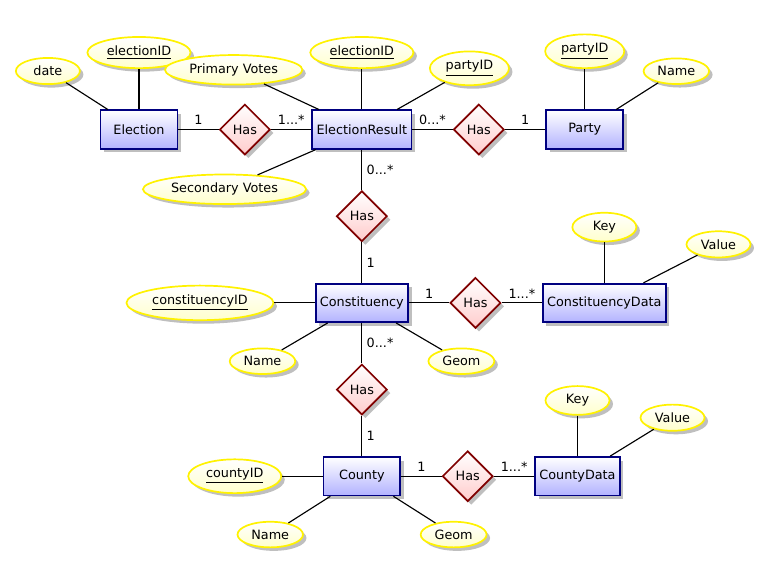
\includegraphics[width=1.1\textwidth]{../img/KIQu2J3.png}
\caption{uml}
\end{figure}

\subsection{Implementation}\label{implementation}

The implementation is structured as a simplified Relational Algebra as well as
the full SQL.

\subsubsection{Election}\label{ImplementationElection}

The \textbf{election} is described by year (\textit{Integer}) and date
(\textit{DateTime}).

\begin{lstlisting}[caption=Election Relational Algebra,numbers=none]
Election(election_ID, date, year)
\end{lstlisting}

\begin{lstlisting}[caption=Election SQL,language=SQL]
CREATE TABLE election
(
  electionid bigint NOT NULL,
  date timestamp without time zone,
  year integer NOT NULL,
  CONSTRAINT election_pkey PRIMARY KEY (electionid)
)
\end{lstlisting}



\subsubsection{Party}\label{ImplementationParty}


The \textbf{party} is described by the name (\textit{String}).

\begin{lstlisting}[caption=Party Relational Algebra,numbers=none]
Party(Party_ID, Name)
\end{lstlisting}


\begin{lstlisting}[caption=Party SQL,language=SQL]
CREATE TABLE party
(
  partyid serial NOT NULL,
  name character(200),
  color character varying(255),
  partyname character varying(255),
  CONSTRAINT party_pkey PRIMARY KEY (partyid)
)
\end{lstlisting}


\subsubsection{County}\label{ImplementationCounty}

The \textbf{county} is described by the name (\textit{String}), number
(\textit{Integer}) and coordinates (\textit{Geom}).


\begin{lstlisting}[caption=County Relational Algebra,numbers=none]
County(County_ID, Name, Nr, coordinates)
\end{lstlisting}



\subsubsection{Constituency}\label{ImplementationConstituency}

The \textbf{constituency} is described by the name (\textit{String}), number
(\textit{Integer}) and coordinates (\textit{Geom}).


\begin{lstlisting}[caption=Constituency Relational Algebra,numbers=none]
Constituency(Constituency_ID, Name, Nr, coordinates)
\end{lstlisting}



\subsubsection{Constituency Data}\label{ImplementationConstituencyData}


The \textbf{constituency data} has a key (\textit{ConstituencyDataKey}) and
value (\textit{Double}):\\

Constituency 1\textless{}-\textgreater{}n
ConstituencyData n \textless{}-\textgreater{} 1 ConstituencyDataKeys


\begin{lstlisting}[caption=Constituency Data and -Keys Relational
Algebra,numbers=none]
ConstituencyData(Constituency_ID, Key_ID, value)
ConstituencyDataKey(Key_ID, name)
\end{lstlisting}



\begin{lstlisting}[caption=Constituency Data SQL,language=SQL]
CREATE TABLE public.constituency_data
(
  gid BIGINT NOT NULL,
  key CHARACTER VARYING(255),
  value BIGINT NOT NULL,
  CONSTRAINT belongs_to_constituency FOREIGN KEY (gid)
      REFERENCES constituency (gid) MATCH SIMPLE
      ON UPDATE NO ACTION ON DELETE NO ACTION
)
\end{lstlisting}



\subsubsection{County Data}\label{ImplementationCountyData}


The \textbf{county data} has a key (\textit{CountyDataKey}) and
value (\textit{Double}): \\

County 1 \textless{}-\textgreater{} n CountyData n \textless{}-\textgreater{}
1 CountyDataKeys


\begin{lstlisting}[caption=County Data and -Keys Relational
Algebra,numbers=none]
CountyData(County_ID, Key_ID, value)
CountyDataKeys(Key_ID, name)
\end{lstlisting}


\begin{lstlisting}[caption=County Data SQL,language=SQL]
CREATE TABLE public.county_data
(
  gid BIGINT NOT NULL,
  key CHARACTER VARYING(255),
  value BIGINT NOT NULL,
  CONSTRAINT belongs_to_county FOREIGN KEY (gid)
      REFERENCES county (gid) MATCH SIMPLE
      ON UPDATE NO ACTION ON DELETE NO ACTION
)
\end{lstlisting}



\subsubsection{Election Results}\label{ImplementationElectionResult}


The \textbf{election result} is identified by \textit{constituency},
\textit{election} and \textit{party}. It gives the number primary votes
(\textit{Integer}) and secondary votes (\textit{Integer}): \\


Constituency 1\textless{}-\textgreater{}n
ElectionResult n\textless{}-\textgreater{}1
Party

\begin{lstlisting}[caption=ElectionResult Relational Algebra,numbers=none]
ElectionResult(Constituency_ID, Party_ID, Election_ID, primaryVotes, secondaryVotes)
\end{lstlisting}



\begin{lstlisting}[caption=ElectionResult SQL,language=sql]
CREATE TABLE electionresult
(
  constituencyid integer NOT NULL,
  partyid integer NOT NULL,
  primaryVotes integer,
  secondaryVotes integer,
  election_electionid bigint,
  CONSTRAINT constituency_fk FOREIGN KEY (constituencyid)
      REFERENCES constituency (gid) MATCH SIMPLE
      ON UPDATE NO ACTION ON DELETE NO ACTION,
  CONSTRAINT election_fk FOREIGN KEY (election_electionid)
      REFERENCES election (electionid) MATCH SIMPLE
      ON UPDATE NO ACTION ON DELETE NO ACTION,
  CONSTRAINT party_fk FOREIGN KEY (partyid)
      REFERENCES party (partyid) MATCH SIMPLE
      ON UPDATE NO ACTION ON DELETE NO ACTION
)
\end{lstlisting}

